\subsection{Matched controls and contribution attribution}

The matched controls use the same batch size (12), number of log-weighted parents (6), initial scale (0.23), scale limits, and learning rates. Global CMA fits one distribution. The two regional controls fit one distribution per normalized region and allocate batches either equally or by the incumbent/reservation rule. Each control initializes the mean from up to four top-ranked points in its domain and samples about that mean.

\begin{center}\begin{minipage}{\linewidth}\centering\small

\TableHere{Matched controls on the original 144 paired tasks and 128 held-out pairs. $\Delta J$ compares RegionCovOpt with the indicated control, using jointly accepted runs.}

\begin{tabular}{@{}lrrrr@{}}\toprule

Control & \multicolumn{2}{c}{Original} & \multicolumn{2}{c}{Held out}\\

 & Accepted & $\Delta J$ (\%) & Accepted & $\Delta J$ (\%)\\\midrule

RegionCovOpt & 142 & +0.000 & 128 & +0.000\\

Original CMA & 140 & -0.432 & 128 & -0.623\\

Matched global & 141 & -0.171 & 127 & -0.509\\

Regional, equal & 142 & -0.352 & 128 & -0.544\\

Regional, adaptive & 144 & -0.032 & 128 & -0.035\\

DE & 144 & -0.424 & 128 & -1.364\\

Uniform & 144 & -6.270 & 128 & -8.744\\

\bottomrule\end{tabular}\end{minipage}\end{center}

\begin{figure}[tb]
\centering
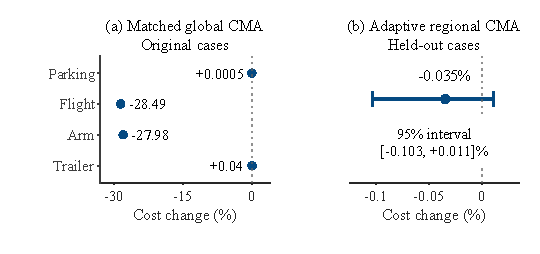
\includegraphics[width=\linewidth]{../figures/attribution.pdf}
\caption{Median paired cost change relative to matched global CMA on the original tasks (a) and adaptively allocated regional CMA on held-out tasks (b). Negative values favor RegionCovOpt. The panels use different horizontal scales. The bar in (b) gives the 95\% scene-cluster bootstrap interval. Only jointly accepted runs enter the comparison.}\label{fig:attribution}
\end{figure}


Figure~\ref{fig:attribution} shows where regional search reduced cost. Flight and manipulation had the largest median gains over matched global CMA. The original-panel median difference narrowed to $-0.032$\% against adaptive regional CMA. The regional controls incorporate both coordinate normalization and region-specific initial means, so this comparison measures their combined effect.

\subsection{Independent selection and held-out task perturbations}

We generated 12 validation tasks and 16 held-out tasks from separate sets of template indices. The perturbations varied the location and size of flight openings, arm goals and obstacles, parking starts and obstacles, and docking starts and aisle geometry. The repository contains the generator, seeds, and inputs.

The original rule led validation with 59 accepted motions in 60 runs. We evaluated five seeds per task and ranked variants first by acceptance count, then by median cost relative to the best accepted candidate for each pair. Removing polling, using diagonal covariance, balancing allocation before feasibility, and combining all three changes yielded 57, 57, 56, and 57 accepted motions, respectively. We fixed the selected rule before testing eight new seeds per held-out task. It and both regional controls returned 128/128 accepted motions. Matched global CMA returned 127/128.

Acceptance therefore favored the full rule on the validation tasks. The held-out cost comparisons below quantify the additional gain over regional CMA.

We estimated a separate 95\% percentile interval for each paired median using 4,000 bootstrap resamples. We resampled whole scenes within each robot family so that the seeds for a scene stayed together. These are marginal intervals for jointly accepted costs.

The held-out median cost change relative to matched global CMA was $-0.509$\% (95\% interval $[-18.400,-0.070]$\%).

The held-out median cost change relative to adaptive regional CMA was $-0.035$\% (95\% interval $[-0.103,0.011]$\%).

The shared initialization produced a motion that passed the planning checks in 125 of 144 original scene--seed pairs within 24 evaluations. This explains much of the early feasibility across optimizers. The budget curves track acceptance by the planner during search. The final cost comparisons use independently verified motions. The repository reports the evaluation count to first feasibility and the complete cost distributions.

\subsection{Representation scope and coverage}

The optimizer transfers across robots through the decoder and evaluator. The parking decoder builds bounded-curvature connections directly or through an intermediate pose. The flight decoder uses ordered rectangular openings, and the arm decoder uses velocity profiles or joint-space knots. The docking decoder uses prescribed gear sequences and aligns the tractor and trailer at the goal. New route branches, joint constraints, or gear sequences may require additional motion families.

At the 960-evaluation budget, each region receives ten independent refreshes after initialization. The probability of reaching a near-optimal motion in these draws depends on how much sampling probability the decoder assigns to that set. Appendix B expresses the bound in terms of that probability. The matched comparisons measure the costs reached at the experimental budget.


Both our C++ implementation of global CMA and pycma 4.5.0 reached objective error below $10^{-8}$ within 12,000 evaluations on all 12 rotated quadratic functions. The problems had dimensions 7, 9, and 13 and condition number $10^3$. Each implementation used its own boundary handling, initial means, and stopping rules. The supplementary records give the final error for each implementation.
